\documentclass[11pt,a4paper]{article}
\usepackage[a4paper,margin=2.2cm]{geometry}
\usepackage{amsmath,amssymb,booktabs,graphicx,float,hyperref,setspace}
\hypersetup{colorlinks=true,linkcolor=blue,urlcolor=blue,citecolor=blue}
\setstretch{1.08}
\setlength{\parskip}{0.55em}
\setlength{\parindent}{0pt}
\newcommand{\ind}{\mathbb{1}}
\title{Selecting a model for Australian government spending projections\\
\large Technical note for internal peer review}
\author{2026 fiscal projection workflow}
\date{24 August 2026}

\begin{document}
\maketitle

\begin{abstract}
This note compares five distinct top-down specifications: structural OLS, levels ARIMAX, differenced ARIMAX, a structural/macro hybrid and an ARDL error-correction model (ECM). The differenced ARIMAX is preferred. It combines economic drivers with the strongest rolling performance and relatively low estimation-window sensitivity. The revised ECM has the best in-sample fit, but exact finite-sample bounds tests do not establish cointegration; it is therefore retained only as a diagnostic sensitivity. Two bottom-up projections are then compared and all specifications are placed in a common framework.
\end{abstract}

\section{Top-down estimates}

\subsection{Data and common treatment}

Let $y_t=G_t^P/Y_t$, where $G_t^P$ is Australian general-government primary fiscal expenditure and $Y_t$ is nominal GDP. The National Accounts numerator comprises government final consumption expenditure, gross fixed capital formation and total income payable, less conventional ``other interest'' payable. Imputed interest on unfunded superannuation liabilities remains in the aggregate. All equations use annual financial-year observations from 1979--80 to 2024--25: 46 observations before model-specific lags.

The demographic block is limited to the population shares aged 0--14 and 65+. Aggregate population is excluded because the outcome is already scaled by aggregate GDP. Separate indicators are used for the three pandemic-affected observations:
\[
D_{j,t}=\ind\{t=j\},\qquad j\in\{2019\text{--}20,2020\text{--}21,2021\text{--}22\}.
\]
The indicators enter every specification in the transformation appropriate to its dependent variable.

PBO consolidated expenses less public debt interest plus net capital investment provide the concept-aligned primary anchor through 2029--30. Thereafter each model supplies cumulative changes:
\[
\widetilde y^{(m)}_t=
\begin{cases}
y_t^{\mathrm{PBO,primary}},&t\leq2030,\\
y_{2030}^{\mathrm{PBO,primary}}+(\widehat y_t^{(m)}-\widehat y_{2030}^{(m)}),&t>2030.
\end{cases}
\]
Model-only paths from the latest National Accounts actual are also reported.

\subsection{Specification 1: structural OLS}

The old-Shapley-style comparison is
\begin{equation}
y_t=\alpha+\boldsymbol\beta'\mathbf a_t+\gamma_T z_t^{\mathrm{tot}}
+\gamma_P z_t^{\mathrm{rp}}+\gamma_u u_t+\boldsymbol\delta'\mathbf D_t+\varepsilon_t,
\end{equation}
where $\mathbf a_t=(a_t^{0\text{--}14},a_t^{65+})'$, $z^{\mathrm{tot}}$ is the standardised terms of trade, $z^{\mathrm{rp}}$ is the standardised relative government-consumption price and $u_t$ is unemployment. This transparent levels equation is useful for attribution; it is not assumed to identify a causal equilibrium.

\subsection{Specification 2: levels ARIMAX}

The same regressors enter a levels regression with stationary ARMA errors:
\begin{align}
y_t&=\alpha+\boldsymbol\beta'\mathbf a_t+\gamma_T z_t^{\mathrm{tot}}
+\gamma_P z_t^{\mathrm{rp}}+\gamma_u u_t+\boldsymbol\delta'\mathbf D_t+n_t,\\
\Phi(L)n_t&=\Theta(L)\epsilon_t.
\end{align}
The selected error process is ARMA$(2,0)$. This model allows serially persistent deviations from the fitted level but does not itself prove that the levels are cointegrated.

\subsection{Specification 3: differenced ARIMAX}

The single reported differenced family is
\begin{align}
\Delta y_t={}&\boldsymbol\beta_a'\Delta\mathbf a_t+\beta_P\Delta z_t^{\mathrm{rp}}
+\theta_0\Delta u_t+\theta_1\Delta u_{t-1}\\
&+\psi_0\Delta z_t^{\mathrm{tot}}+\psi_1\Delta z_{t-1}^{\mathrm{tot}}
+\boldsymbol\delta'\mathbf D_t+n_t,\\
\Phi(L)n_t={}&\Theta(L)\epsilon_t.
\end{align}
This replaces the former duplication between a mechanically differenced ARIMAX and ``dynamic differences''. Changes in unemployment and the terms of trade are used so a permanently high level does not mechanically generate repeated spending growth. The selected residual process is white noise.

\subsection{Specification 4: structural/macro hybrid}

The slow-moving level is
\begin{equation}
y_t^S=\alpha+\boldsymbol\beta'\mathbf a_t+\gamma_Pz_t^{\mathrm{rp}}
+\boldsymbol\delta'\mathbf D_t+e_t^S.
\end{equation}
For $r_t=\Delta y_t-\Delta\widehat y_t^S$, the macro block is
\begin{equation}
r_t=\theta_0\Delta u_t+\theta_1\Delta u_{t-1}
+\psi_0\Delta z_t^{\mathrm{tot}}+\psi_1\Delta z_{t-1}^{\mathrm{tot}}+\eta_t.
\end{equation}
The projected change is $\Delta\widehat y_t^S+\widehat r_t$. Real GDP per capita is not forced into this equation.

\subsection{Specification 5: augmented-Mann ARDL/ECM}

The literature suggests two common Wagner-law formulations: log real expenditure against log real output, and the Mann/Musgrave form relating the log spending share to log real income per person. Because this exercise directly projects spending/GDP, the latter is the closer match. Define
\[
w_t=\log(G_t/Y_t),\qquad q_t=\log(\text{real GDP per capita}),\qquad
p_t=\log(P_t^G/P_t^Y).
\]
The candidate long-run equation is
\begin{equation}
w_t=\alpha+\beta_q q_t+\beta_p p_t+e_t.
\end{equation}
The unrestricted ECM is
\begin{align}
\Delta w_t={}&c+\lambda w_{t-1}+\theta_q q_{t-1}+\theta_p p_{t-1}
+\rho\Delta w_{t-1}\\
&+\sum_i\pi_i\Delta q_{t-i}+\sum_i\kappa_i\Delta p_{t-i}
+\sum_i\mu_i\Delta u_{t-i}+\sum_i\tau_i\Delta z_{t-i}^{\mathrm{tot}}
+\boldsymbol\delta'\mathbf D_t+\epsilon_t.
\end{align}
BIC selects between maximum lag orders one and two; it selects one in the current sample. Age shares are excluded from the cointegrating vector because earlier unit-root checks on these very smooth series were inconclusive and flagged a possible I(2) age-65 series. Unemployment and the terms of trade are short-run conditioning variables only.

\subsection{Relative fit}

\begin{table}[H]
\centering
\caption{Fit, rolling forecasts and projection stability}
\small
\begin{tabular}{lrrrrr}
\toprule
Model & In-sample & Average rolling & 1-year & 5-year & Max window\\
 & RMSE & RMSE & RMSE & RMSE & shift\\
\midrule
Structural OLS & 0.77 & 4.66 & 3.39 & 5.92 & 5.59\\
Levels ARIMAX & 0.55 & 4.45 & 3.18 & 5.69 & 5.10\\
Differenced ARIMAX & 0.59 & 3.58 & 1.80 & 4.97 & 1.39\\
Hybrid & 0.62 & 4.34 & 3.21 & 5.60 & 5.38\\
ARDL ECM & 0.52 & 3.15 & 1.86 & 3.94 & 1.45\\
\bottomrule
\end{tabular}
\begin{flushleft}\footnotesize RMSE and window shifts are percentage points of GDP. Rolling forecasts use origins 2009--10 to 2019--20 and horizons one to five years, conditional on subsequently observed driver paths.\end{flushleft}
\end{table}

The ECM's forecast metrics are promising, but a long-run model cannot be selected on predictive fit alone: cointegration is a maintained requirement. Among the specifications that do not require a validated level equilibrium, the differenced ARIMAX has the lowest average rolling RMSE and much lower pre-COVID endpoint sensitivity than the three level-based alternatives.

\begin{figure}[H]
\centering
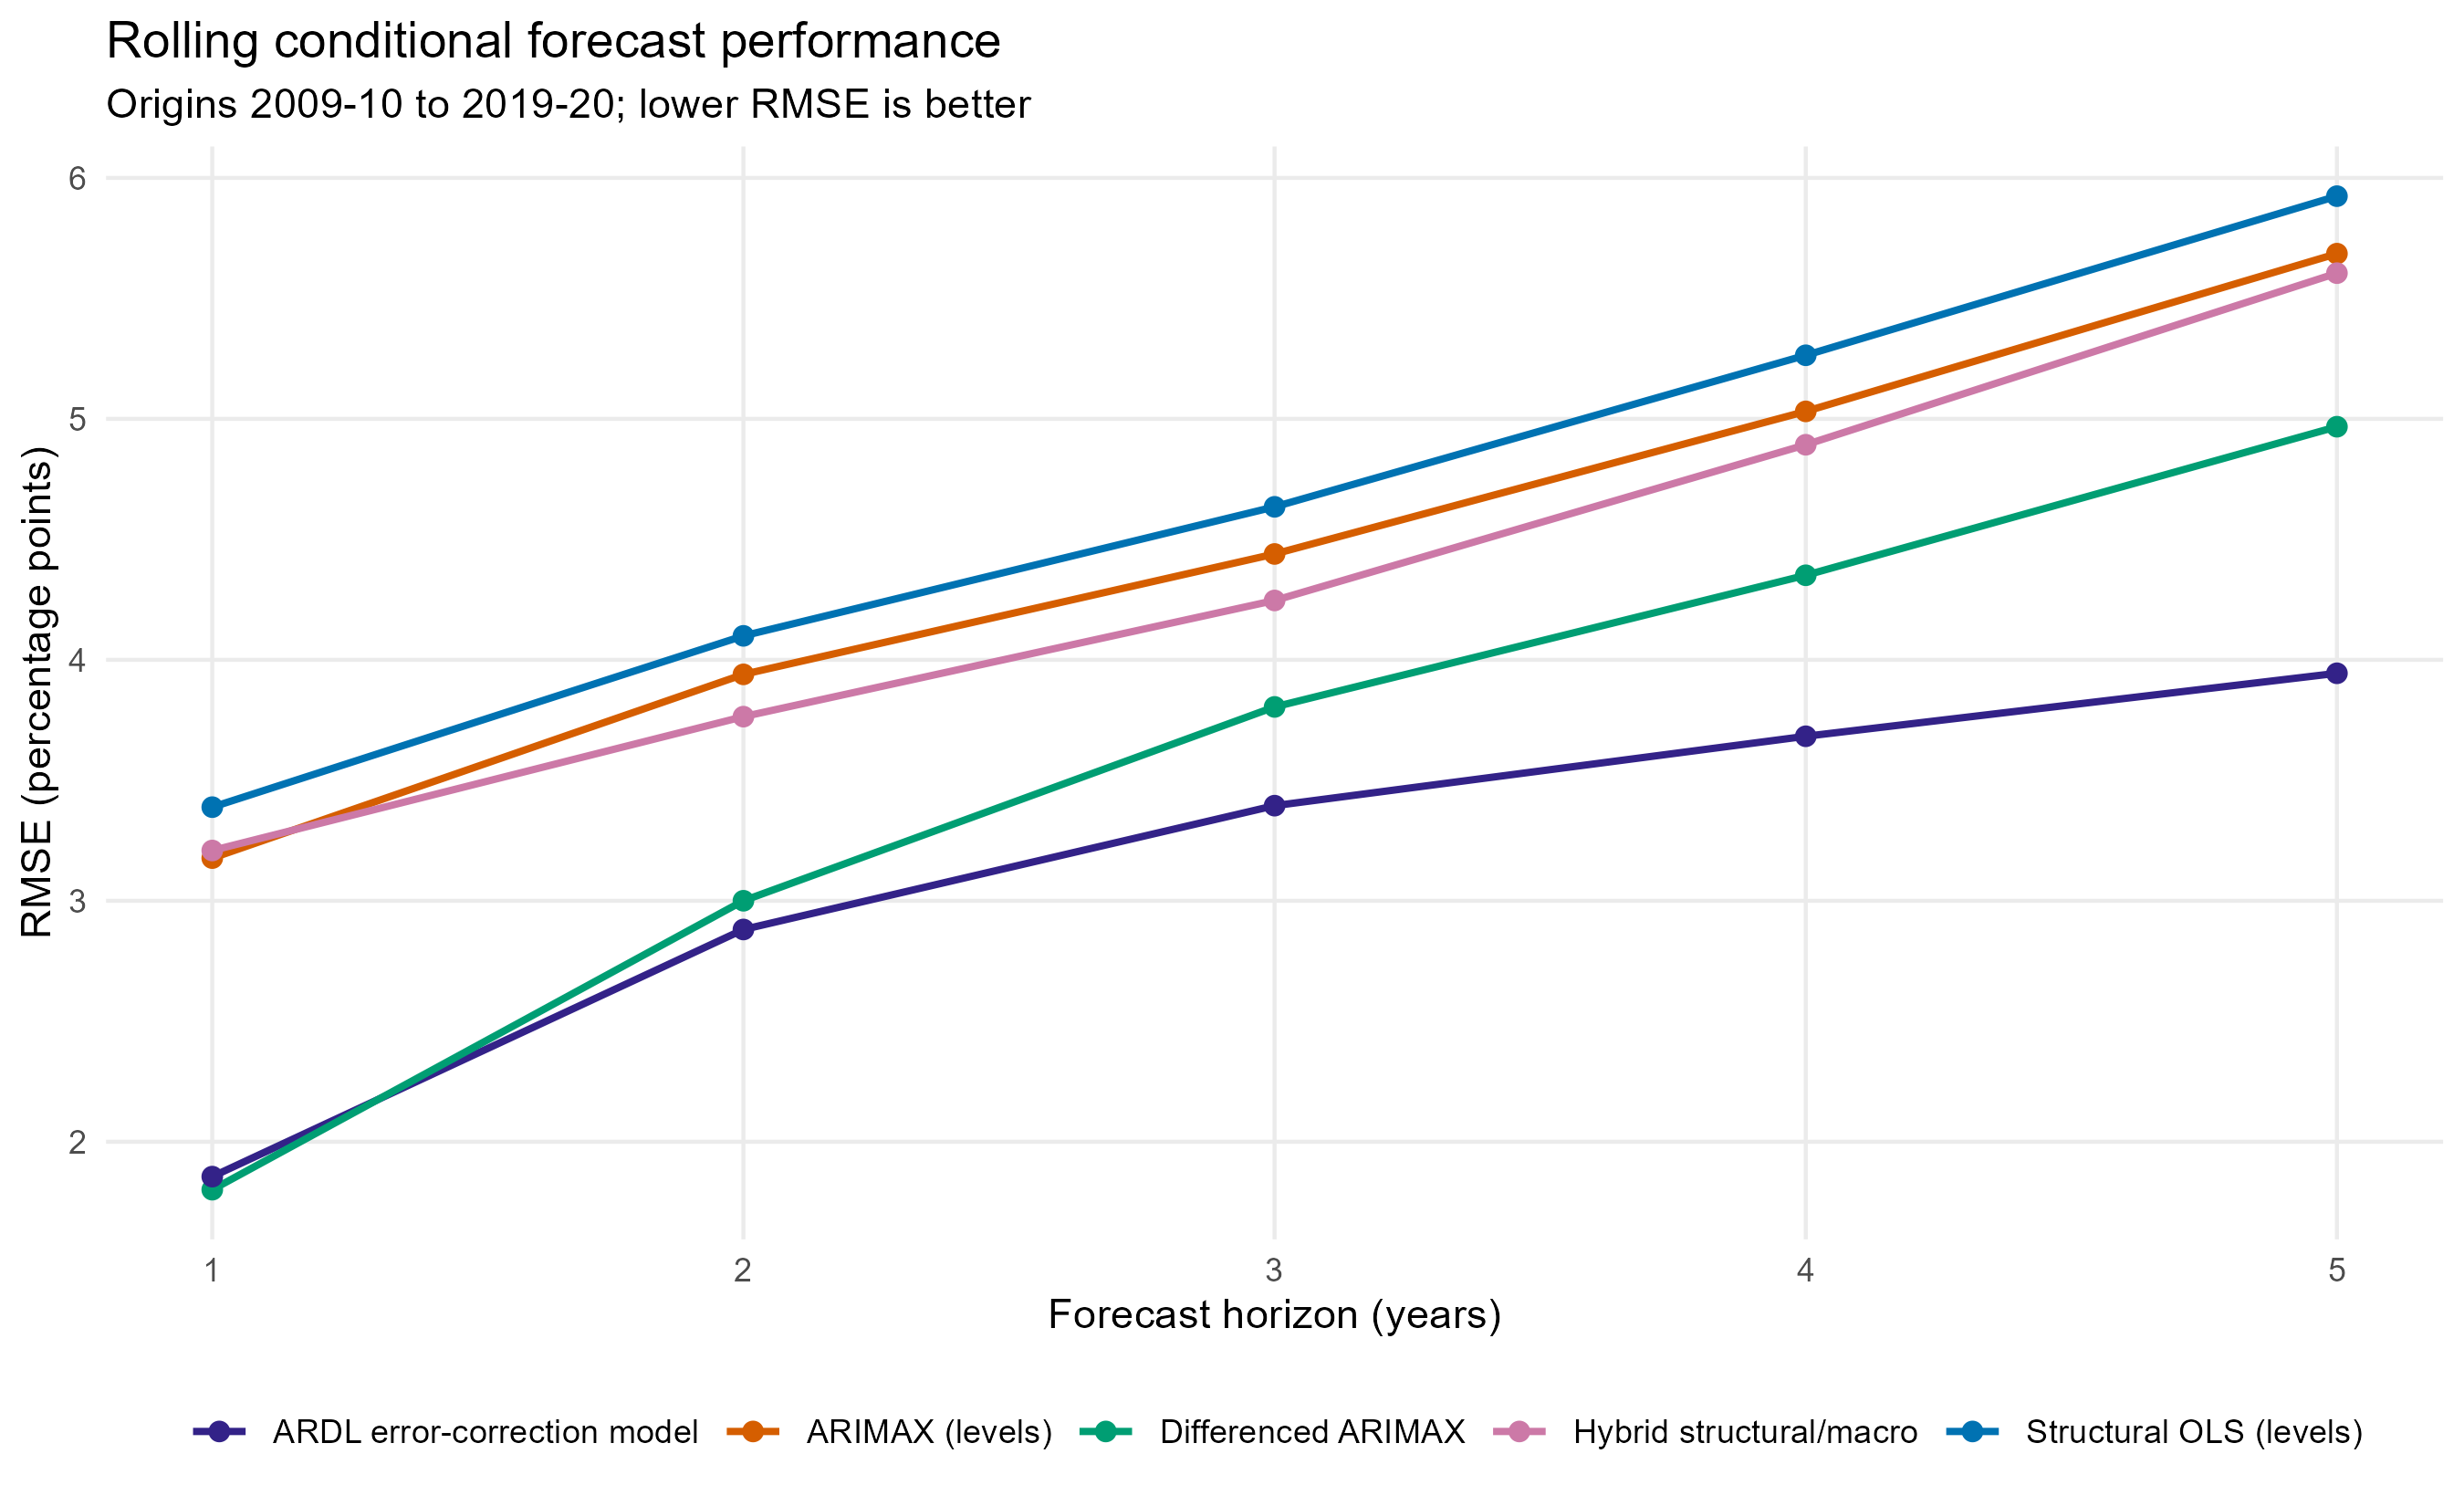
\includegraphics[width=.94\textwidth]{figures/five_model_rolling_rmse.png}
\caption{Rolling conditional forecast RMSE.}
\end{figure}

\subsection{Cointegration and ECM validation}

ARDL bounds inference permits a mixture of I(0) and I(1) regressors but not I(2) variables \cite{pss}. ADF and KPSS tests on first differences give no I(2) warning for $w_t$, $q_t$ or $p_t$. Zivot--Andrews tests are also reported to allow one endogenous level/trend break.

With conventional interest excluded, the exact finite-sample Case III bounds results are:
\begin{itemize}
\item joint lagged-level F statistic $2.298$, below the 5 per cent I(0) bound $4.062$ (exact $p=0.438$);
\item lagged-dependent-level t statistic $-1.560$, above the I(0) bound $-2.904$ (exact $p=0.675$); and
\item augmented-ARDL F statistic for the lagged independent levels $1.557$ ($p=0.225$).
\end{itemize}
The first two tests support no cointegration and the third does not rule out a degenerate-regressor case. The estimated adjustment coefficient becomes more negative, $\widehat\lambda=-0.152$, but remains insignificant ($p=0.128$). Breusch--Godfrey, RESET, Breusch--Pagan and recursive CUSUM tests do not reject at 5 per cent, but satisfactory conditional residual checks cannot replace the missing level relationship. A one-break diagnostic for the candidate long-run regression selects 2018--19, which adds to the stability concern.

The ECM is therefore rejected as the primary long-run projection model. It remains in the comparison as a disciplined test of the economic hypothesis, not as evidence that the hypothesis holds.

\subsection{Preferred top-down approach}

The preferred top-down model is the differenced ARIMAX. It includes the limited demographic block, relative prices and cyclical macro drivers without relying on an unsupported cointegrating relationship. Its PBO-anchored 2065--66 primary fiscal-expenditure endpoint is 32.94 per cent of GDP, compared with 31.71 for the rejected ECM, 36.27 for levels ARIMAX, 36.16 for the hybrid and 36.52 for structural OLS. Public debt interest is added separately from the projected debt stock and effective interest-rate assumptions when constructing total expenditure and debt paths.

\begin{figure}[H]
\centering
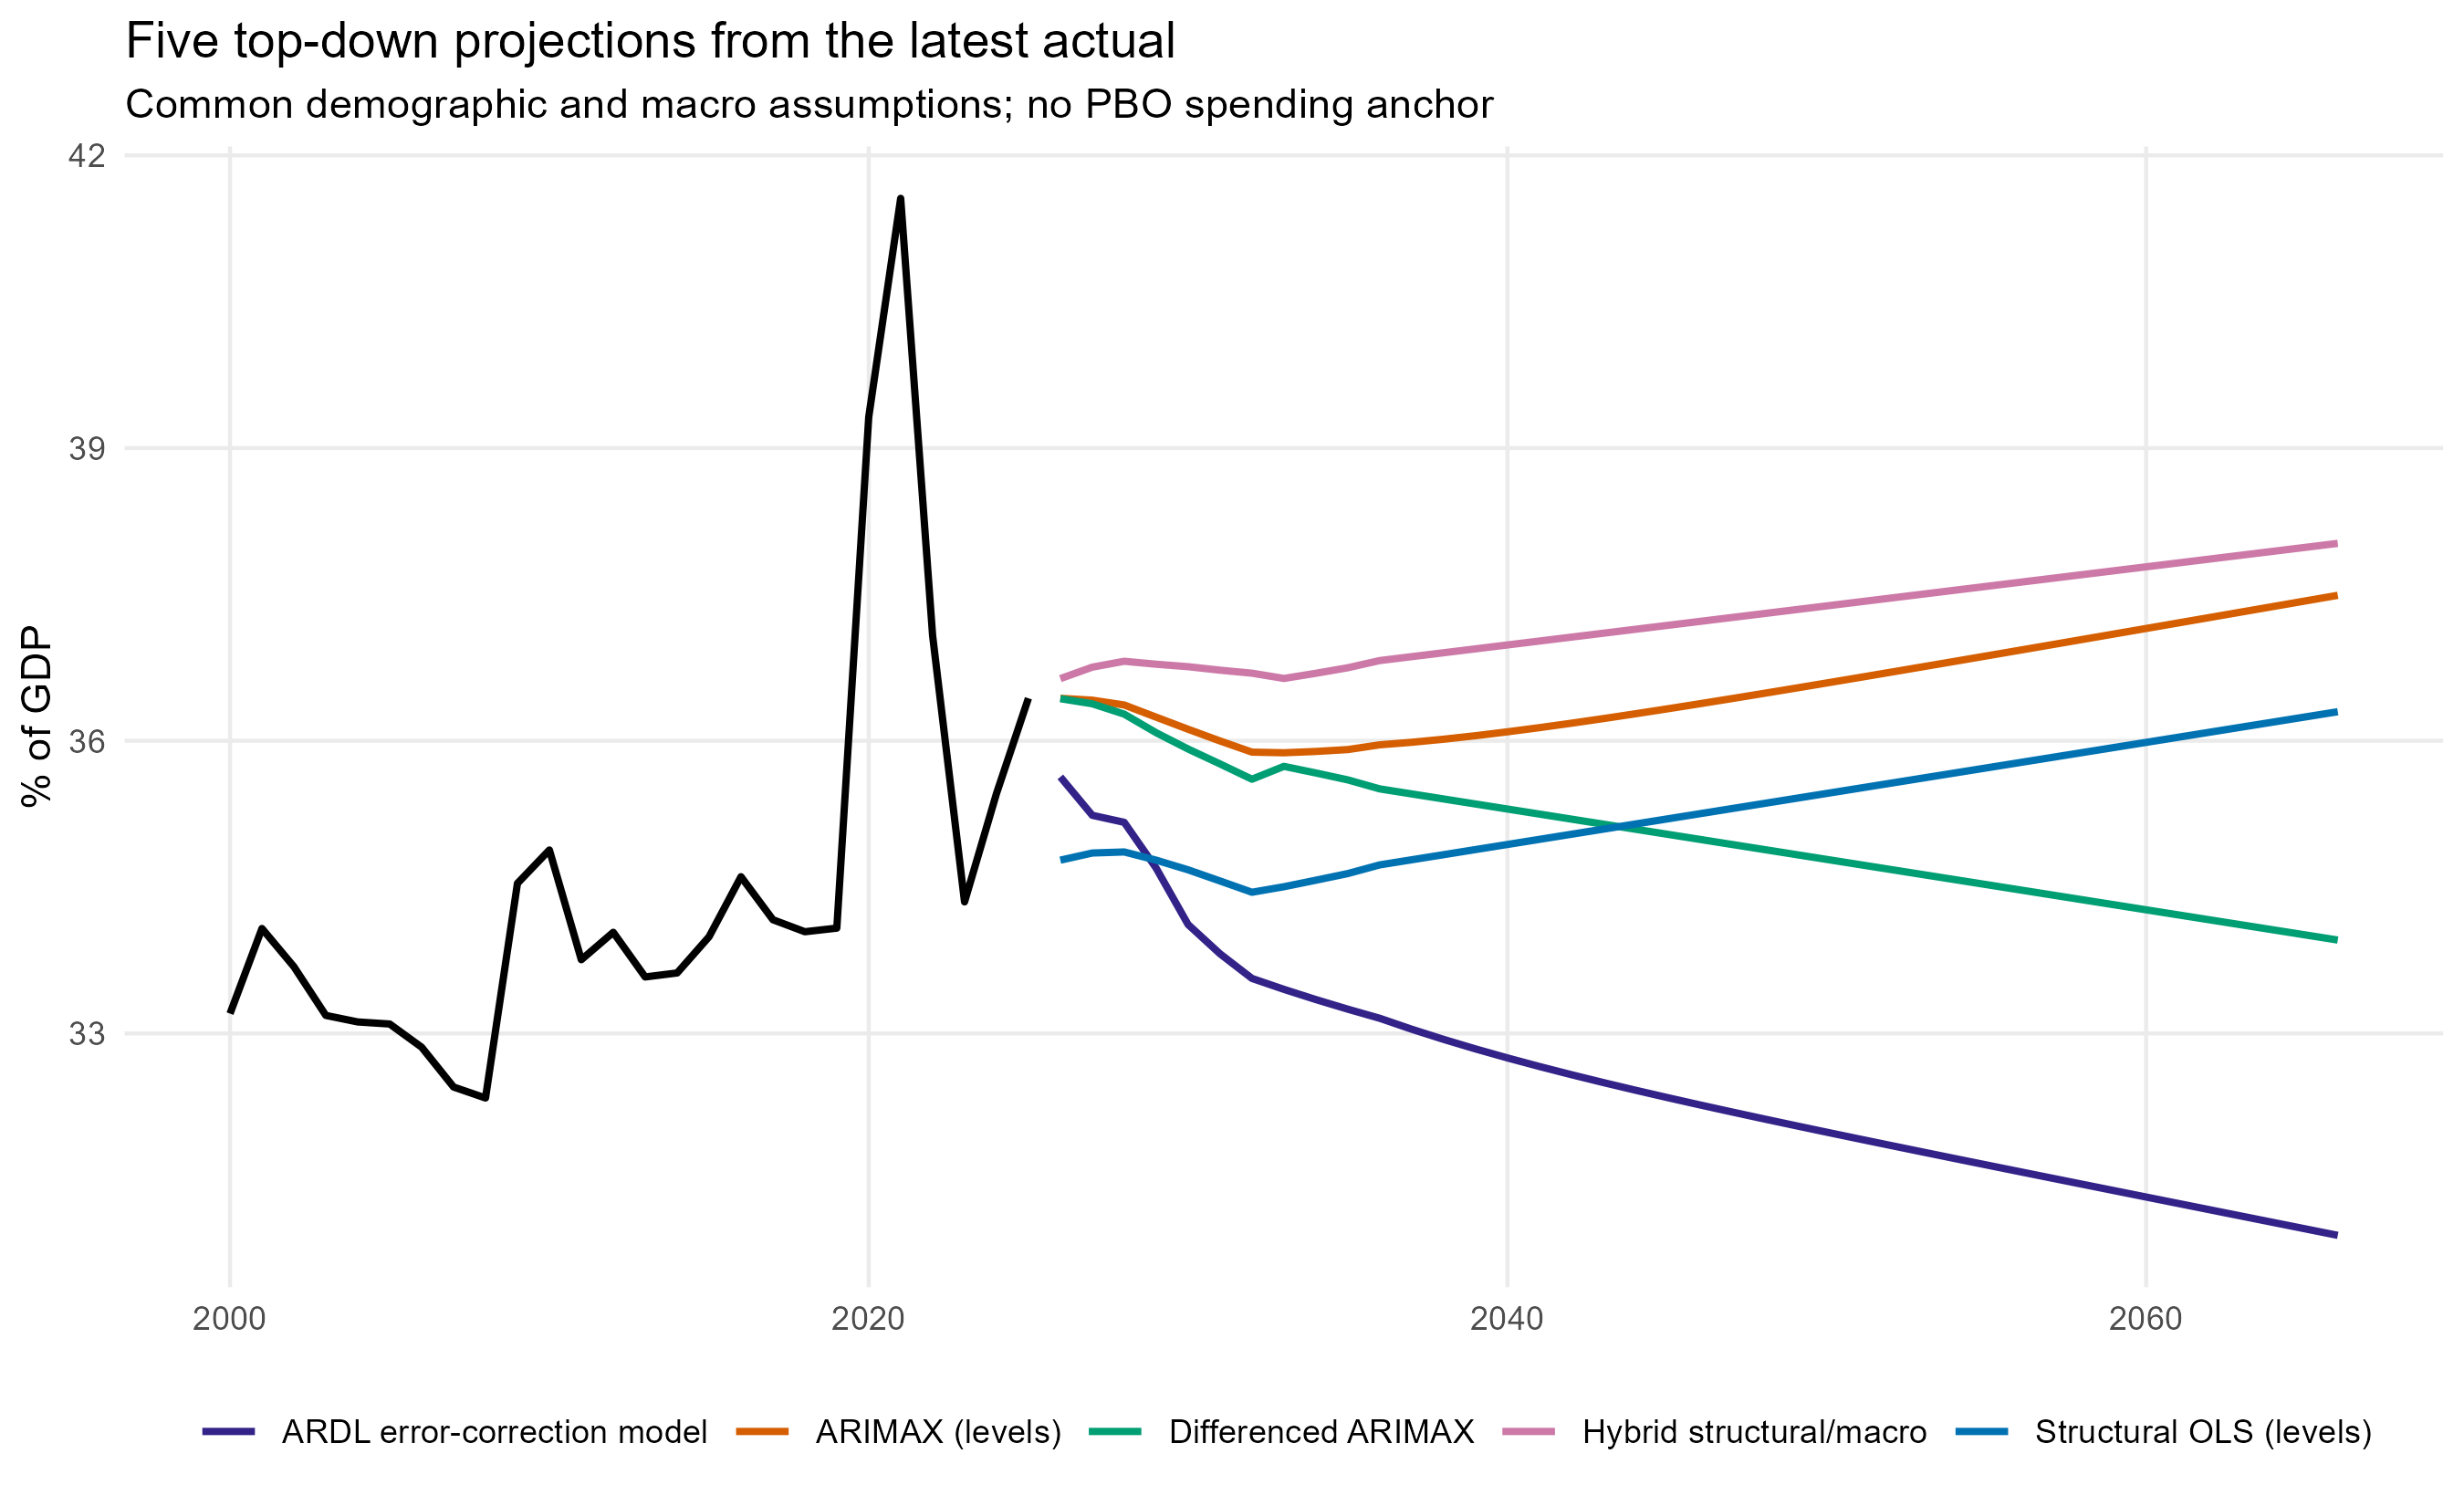
\includegraphics[width=.94\textwidth]{figures/five_model_paths_model_only.png}
\caption{Model-only projections beginning from the latest National Accounts actual.}
\end{figure}

\begin{figure}[H]
\centering
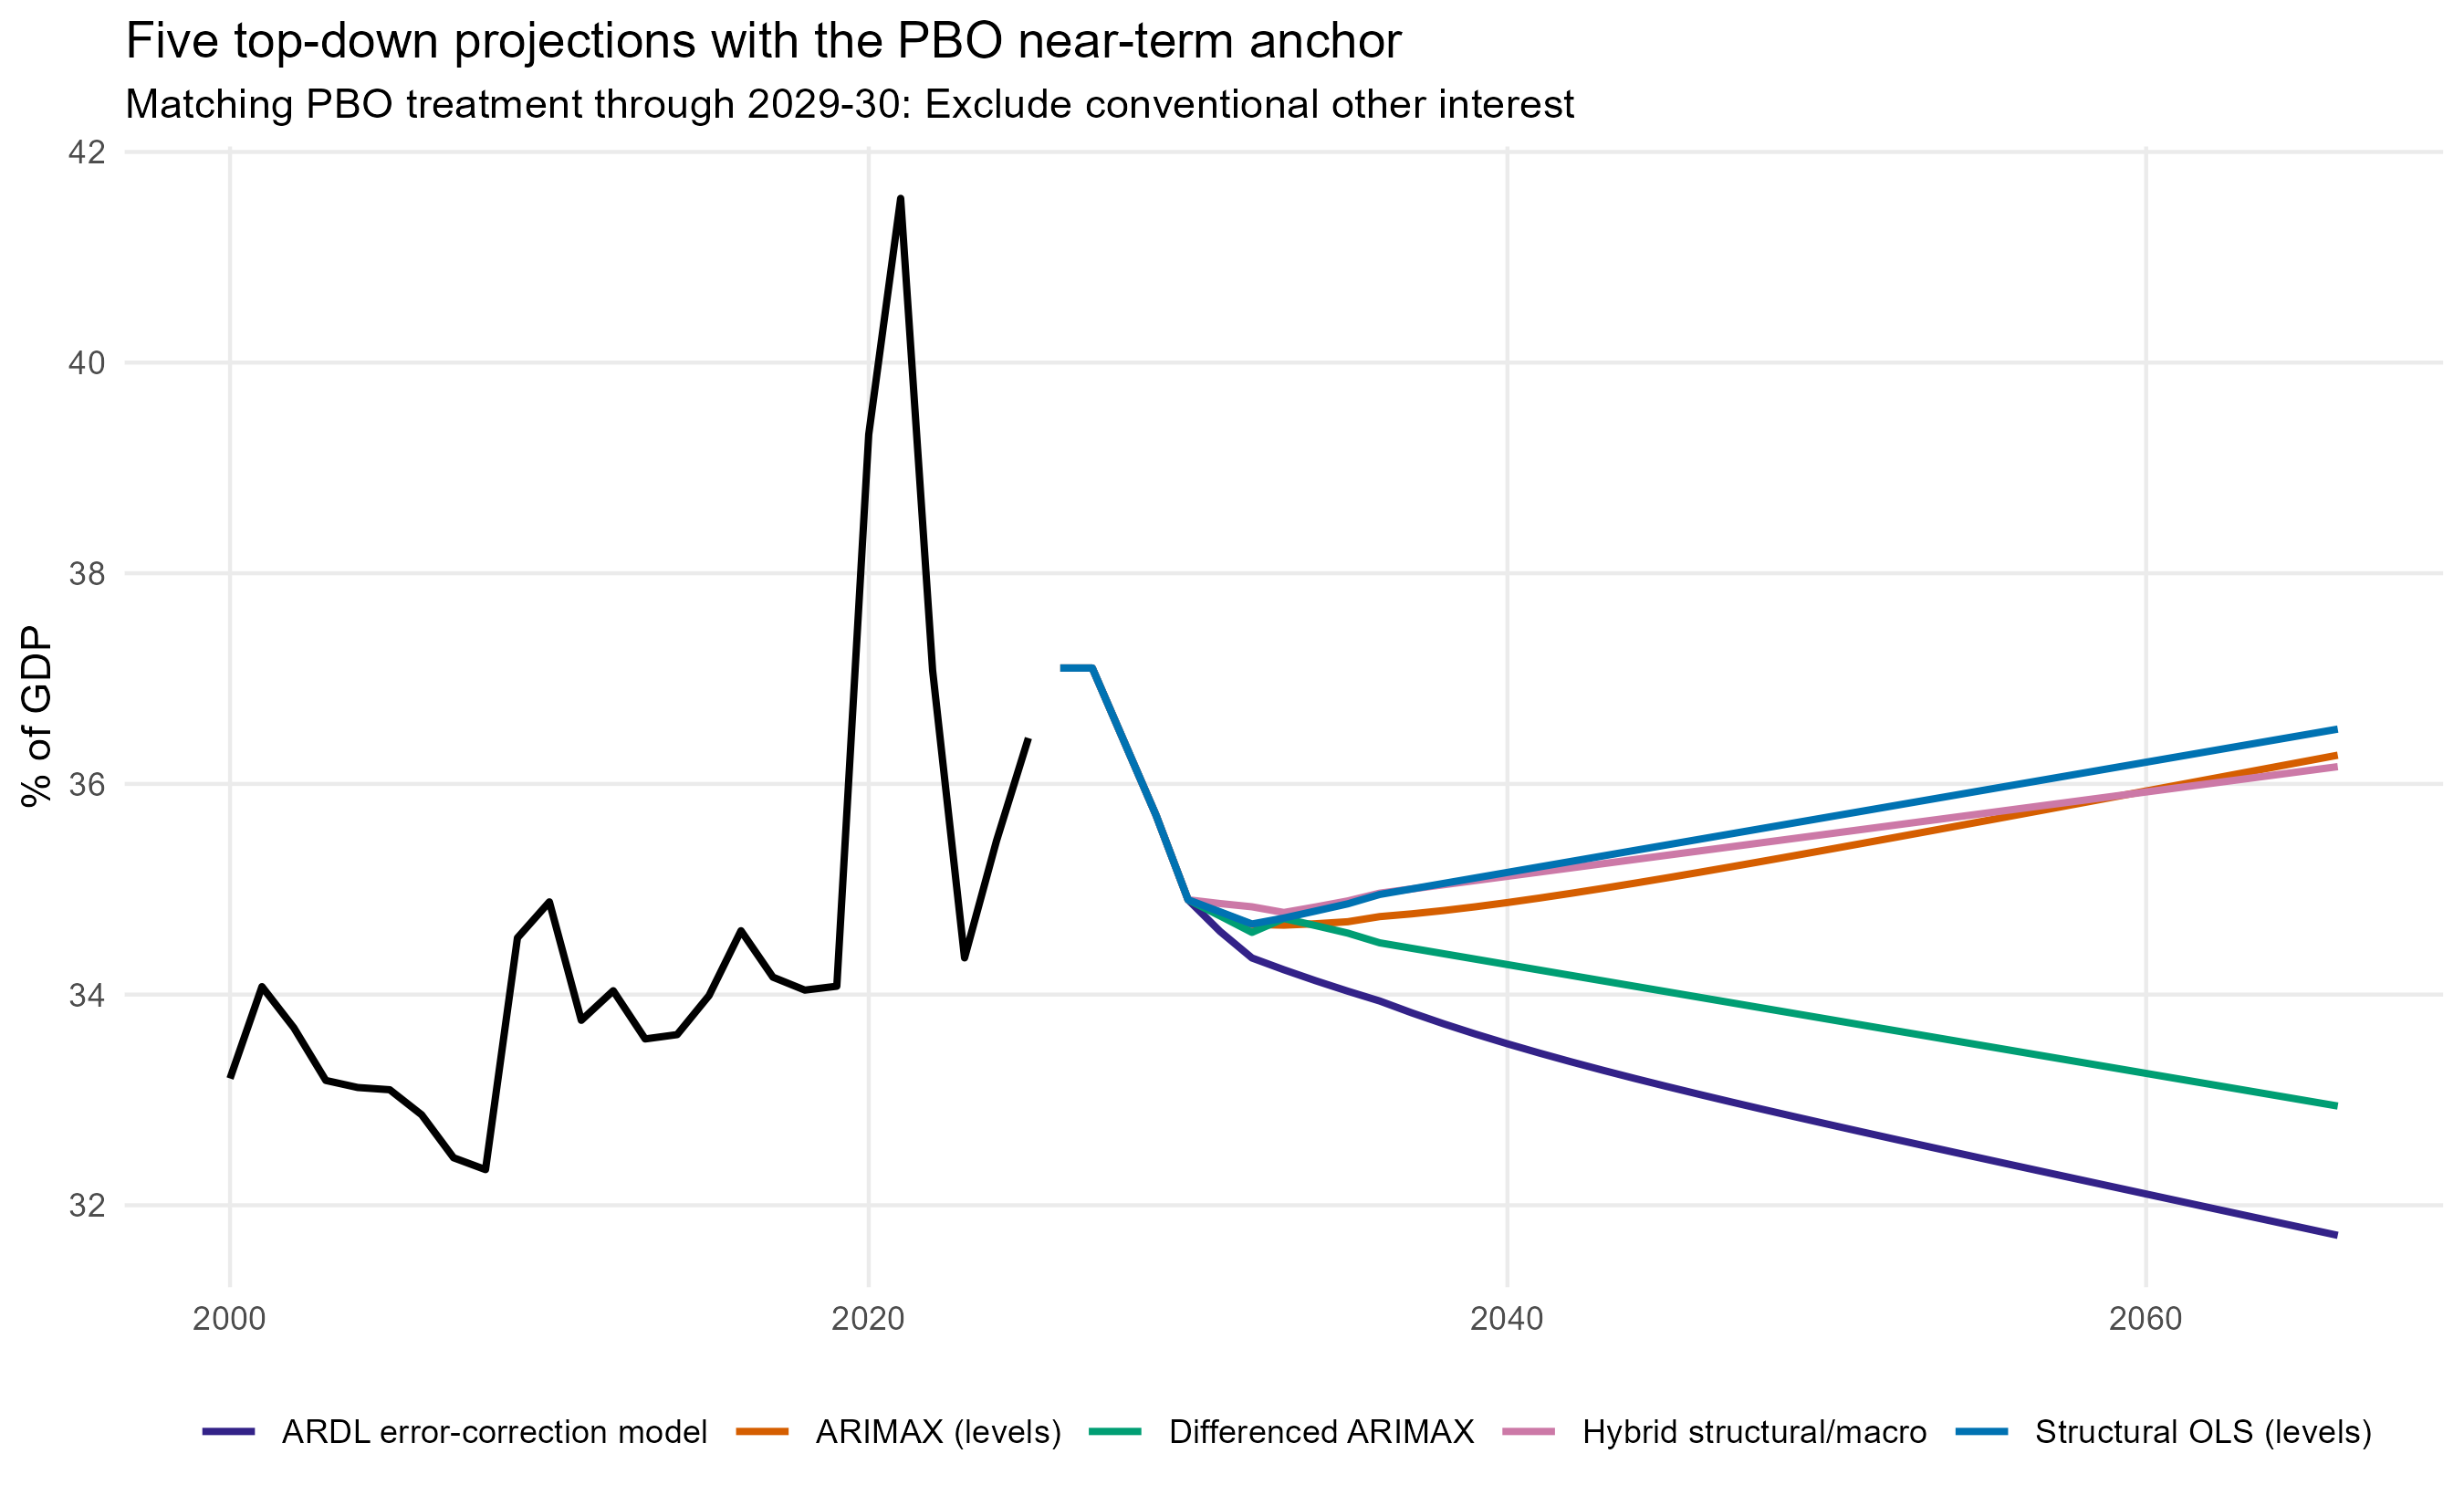
\includegraphics[width=.94\textwidth]{figures/five_model_paths_pbo_anchor.png}
\caption{PBO expenses less public debt interest plus net capital investment through 2029--30, followed by model changes.}
\end{figure}

\section{Literature background}

The public-spending time-series literature provides a useful structure but not a universal specification. Akitoby et al. separate short-run expenditure dynamics from a long-run output relation and survey Wagner-type formulations \cite{akitoby}. Arpaia and Turrini use error-correction methods for government expenditure in European economies \cite{arpaia}. For a spending-share outcome, the Mann/Musgrave formulation motivates $w_t$ and $q_t$. Relative public-sector prices are included because labour-intensive public services can become more expensive relative to aggregate output prices \cite{price}.

Pesaran, Shin and Smith provide the ARDL bounds framework \cite{pss}. Sam, McNown and Goh show that the joint F test should be supplemented by tests of the lagged dependent and independent levels to exclude degenerate cases \cite{sam}. Published Australian Wagner-law evidence is mixed and period-dependent \cite{australia}. Consequently, cointegration and stability are treated as requirements for the ECM, not inferred from a high $R^2$ or low in-sample RMSE.

\section{Bottom-up approaches}

The fixed demographic-rate baseline projects each function from its observed level using a transparent exposure rule. Defence follows an exogenous share-of-GDP policy path. Health, education and social protection respond to relevant age structure. Health also has central excess cost growth of 0.75 per cent per year above the common nominal cost base. This represents technology, intensity, wages and relative-price pressure not explained by demographics and general inflation. It is a scenario assumption informed by the Australian Intergenerational Report, PBO projections, OECD health-spending work and Productivity Commission evidence, not a precisely estimated structural coefficient.

The data-enhanced sensitivity uses the same exposure and policy structure but adds public relative-price information and a shrunk historical category-intensity residual. The estimate is capped, shrunk toward the baseline and partly damped by 2040 to avoid extrapolating COVID disruption, classification changes or a short noisy history. The fixed-rate model remains the baseline because it is more transparent; the enhanced path tests sensitivity.

\section{Using all specifications together}

The PBO-anchored differenced ARIMAX is the preferred empirical top-down projection. Structural OLS supports old-Shapley attribution. Levels ARIMAX and the hybrid show the consequences of imposing slow-moving levels relationships. The ECM provides a formal long-run income test, but its current failure is informative and should remain visible. The fixed-rate bottom-up path explains functional spending pressures, while the data-enhanced bottom-up path tests relative-price and excess-cost assumptions. These paths should not be averaged mechanically: disagreement is model uncertainty.

\begin{thebibliography}{9}
\bibitem{akitoby} Akitoby, Clements, Gupta and Inchauste, \emph{Public Spending, Voracity, and Wagner's Law in Developing Countries}, IMF Working Paper 04/202, \url{https://www.imf.org/external/pubs/ft/wp/2004/wp04202.pdf}.
\bibitem{arpaia} Arpaia and Turrini, \emph{Government Expenditure and Economic Growth in the EU}, \url{https://www.bancaditalia.it/pubblicazioni/altri-atti-convegni/2007-fiscal-policy/Arpaia_Turrini.pdf?language_id=1}.
\bibitem{pss} Pesaran, Shin and Smith (2001), \emph{Bounds testing approaches to the analysis of level relationships}, \url{https://onlinelibrary.wiley.com/doi/pdf/10.1002/jae.616}.
\bibitem{sam} Sam, McNown and Goh (2019), \emph{An augmented autoregressive distributed lag bounds test for cointegration}, \url{https://www.sciencedirect.com/science/article/pii/S0264999318307843}.
\bibitem{australia} \emph{Wagner's law in Australia: a structural time series analysis}, \url{https://www.tandfonline.com/doi/full/10.1080/00036846.2016.1203063}.
\bibitem{price} \emph{Government Spending and Relative Prices}, \url{https://journals.sagepub.com/doi/10.1177/1091142103031003002}.
\end{thebibliography}

\end{document}
